

\documentclass[11pt,a4paper]{article}
\usepackage{graphics}
\usepackage{subfigure} 
\usepackage{epsfig}
\usepackage{color}
\usepackage{times,mathptm}
\usepackage{color}
\usepackage{graphicx}
\usepackage{wasysym}
\usepackage{comment}
\usepackage{listings}
\usepackage[T1]{fontenc}
\usepackage{lipsum}
\renewcommand{\baselinestretch}{1.07}
\topmargin= -0.4in
\textheight = +8.9in
\oddsidemargin = 0.05in
\evensidemargin = 0.05in
\textwidth = 6.5in



\title{Some Basic SIR Models with Variations}
\author{Hsiang Wang, Shenghan Mei, Xinyu Shi}

\begin{document}
\maketitle


\begin{abstract}


\noindent	
 This paper introduces SIR models of Covid-19 with some variations. First, we introduce some notations for SIR models. Then we discuss agent-based and ODE/PDE models in one-dimension and two-dimension respectively with some proper simulations. Last but not least, we show our extensions to the SIR models including simulating elementary schools disease spreading, reinfection and masks wearing situations. 

\end{abstract}

\section*{Introduction}

   SIR model shows how disease spreads through a population. People are in one of three states at time t:

$s(t)$: the number of susceptible population in the total population at time t.

$i(t)$: the number of infectious population in the total population at time t.

$r(t)$: the number of removed population in the total population at time t.

The model is characterized by the following system of differential equations:

$\frac{ds}{dt} = -b \times s(t) \times i(t)$

$\frac{dr}{dt} = k \times i(t)$

$\frac{di}{dt} = b \times s(t) \times i(t) - k \times i(t)$

$b$ represents the number of interactions for each individual per day 

$k$ represents the recovery rate from the diesease

There are some more parameters:

$N$ : Total number of people in a population

$T$ : Time duration

$ii$ : initial fraction of population been infected

\medskip \noindent
The ultimate purpose for a model is to serve for real world application, and coronavirus is the best example we can use and extremely care recently. One extension model we propose is to apply our basic SIR model into simulating elementary schools situation to decide whether the school should reopen or not. What I propose is to input the N(population) as the average elementary school students, I(Infectious people) and R(recovered people) to the model, as well as the average k(recover rates) from research as a baseline. After that, we can change the b(contact people) to observe what is the trend for number of infectious people. At last, we will give our conclusions and some improvements to our model. 


\medskip \noindent
Secondly, it is likely for people to be reinfected if people are not immune to the disease after they are recovered. Therefore, we could implement reinfection into the SIR model. For Agent-Based model, this could be implemented by adding probability of reinfection, where reinfected people would be infected again. Alternatively, we could let people who are recovered becomes susceptible with certain probability. In addition, we could add a new variable immunization. This variable stores the probability of been immunized from the disease. For example, immunization = 0.2 means 80\% chance of been reinfection. The value increases if individuals recover from the disease. For ODE model, this could be implement by adding probability of reinfection r. This has the form: 

$$\frac{ds}{dt} = -b \times s(t) \times i(t)$$

$$\frac{dr}{dt} = k \times i(t) - r \times r(t)$$

$$\frac{di}{dt} = b \times s(t) \times i(t) - k \times i(t) + r \times r(t)$$


\medskip \noindent
It is obvious that people wearing masks can slow down the disease spread. We can know that most of Chinese people wore face masks and the actual numbers of infections have decreased at a greater rate (Cooper et al). Therefore, we could implement the effect of the use of masks into the SIR model. For ODE model, we can implement it by reducing the parameter b. We can obtain data from to calculate the efficiency of the use of masks on the number of interactions each day that could spread the disease. Thus, we can judge whether the use of masks can slow down the spread of the virus.


\section*{Some SIR models }
\subsection*{Basic SIR models}
{Agent-based model}:

\medskip \noindent
The key idea is that we have total number of N people and some of them are infected initially. These N people interact with b other people per day. If the person is infectious, the person who interacts with him will get infected, which can be done by the discrete method. Later, we introduce k, which is the probability of a person gets recovered. We can choose the duration we want to simulate in the model.

\medskip \noindent
ODE model:

\medskip \noindent
This model treats SIR model as initial value problem. s(t), i(t), r(t) as fraction of population with $s(t)+i(t)+r(t)=1$ for this model. We could apply $solve_{ivp}$ from scipy to solve. The parameters are $b$,$k$, $N$ and $ii$.

\medskip \noindent
We fixed parameters for these simulation:
\newline
- number of days = 40
\newline
- percentage of initial infected people = 0.01
\newline
- number of people = 1000

\newpage
  \begin{center}
 	Figure 1: First Simulation models with b=1, k=1/3
 \end{center}

 \begin{center}
 	
 	\begin{tabular}{c c}
 		\textbf{\underline{Continuous}} &
 		\textbf{\underline{Discrete}} \\
 		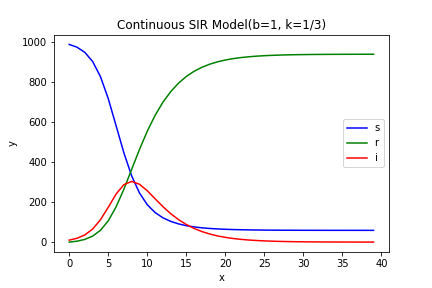
\includegraphics[width=7cm, height=5.5cm]{C_SIR_1.png} & 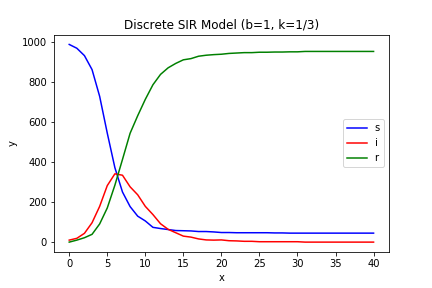
\includegraphics[width=7cm,height=5.5cm]{D_SIR_2.png}
 	\end{tabular}
 
 \end{center}

\medskip \noindent
For these models, the number of susceptible people decreases exponentially until day 18 at about 70 and then keeps no change. The number of infectious people peaks at about day 9 and decrease to 0 after day 26, which is also the time that recovery people stays at about 930 after an exponential raise. 


%**The second simulation is b=5, k=0.2**

  \begin{center}
 	Figure 2: Second Simulation models with b=5, k=0.2
 \end{center}

 \begin{center}
 	
 	\begin{tabular}{c c}
 		\textbf{\underline{Continuous}} &
 		\textbf{\underline{Discrete}} \\
 		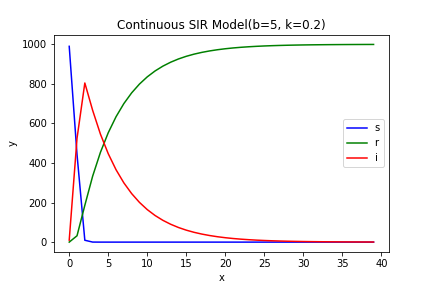
\includegraphics[width=.5\textwidth]{C_SIR_2.png} & 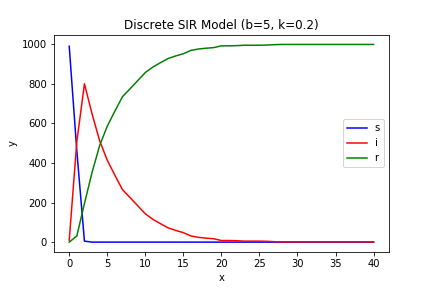
\includegraphics[width=.5\textwidth]{D_SIR_1.png}
 	\end{tabular}
 
 \end{center}

\medskip \noindent
In this case, because of number of contact people increase to 5, the number of infectious people reaches its peak at the first few days with approximately 820 people. This leads to number of susceptible people drops to 0 within 3 days. The rate of recovery is relatively slow compare with the rate of infected. It takes around 24 days to recover every patient. 

\medskip \noindent
These simulations demonstrate discrete and continuous models are very similar. There are few points in the graph are not smooth is due to calculation errors from the randomness in the discrete model.

\newpage
  \begin{center}
 	Figure 3: Phase for Susceptible
 \end{center}

 \begin{center}
 	
 	\begin{tabular}{c c}
 		\textbf{\underline{Continuous}} &
 		\textbf{\underline{Discrete}} \\
 		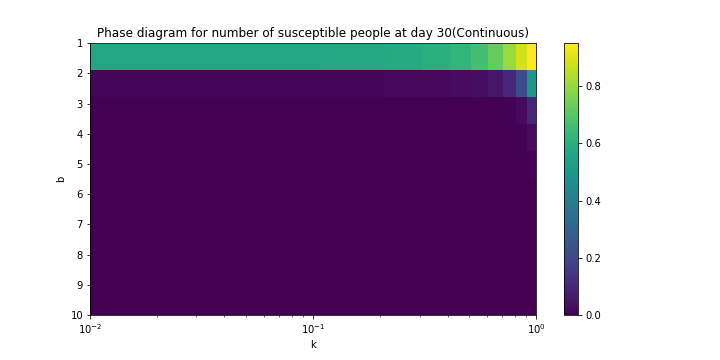
\includegraphics[width=.5\textwidth]{Phase_Continuous_S.png} & 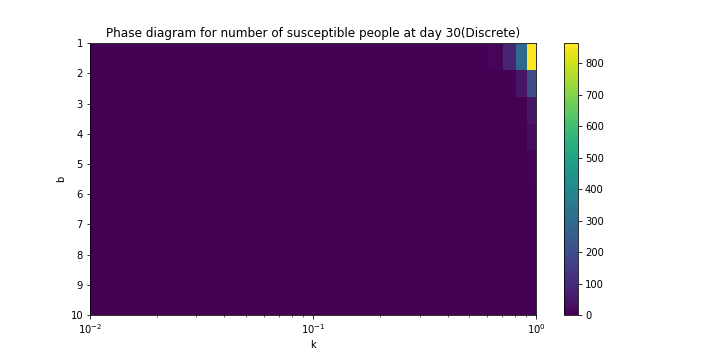
\includegraphics[width=.5\textwidth]{Phase_Discrete_S.png}
 	\end{tabular}
 
 \end{center}
\medskip \noindent
It is no hard to observe that at day 30, both models illustrate that the susceptible people are about zero in most situations with some exceptions, mainly case b = 1 in continuous model and b = k = 1 in discrete model. This should not be surprising since more people they interact with (b increases), it takes shorter time to spread the disease. At day 30, almost the entire population has already gotten. 


  \begin{center}
 	Figure 4: Phase for Infectious
 \end{center}
 \begin{center}
 	
 	\begin{tabular}{c c}
 		\textbf{\underline{Continuous}} &
 		\textbf{\underline{Discrete}} \\
 		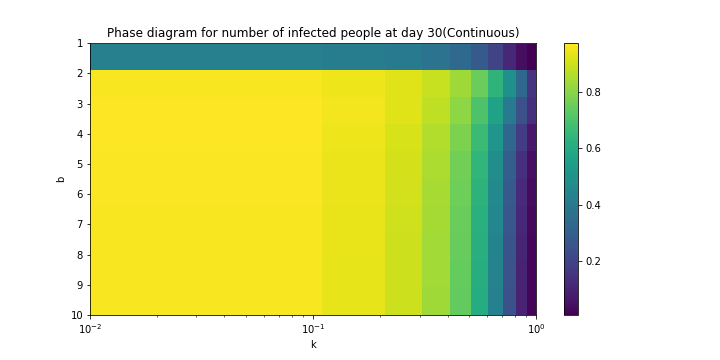
\includegraphics[width=.5\textwidth]{Phase_Continuous_I.png} & 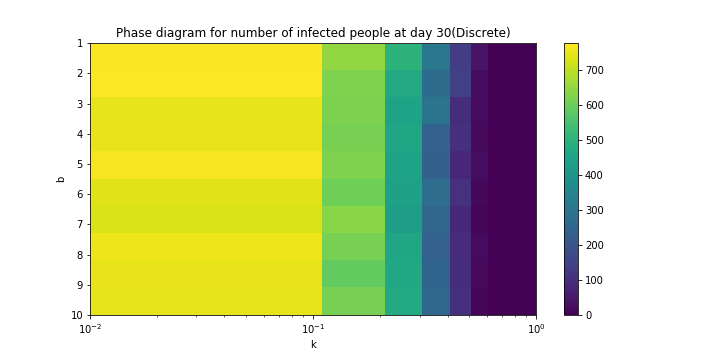
\includegraphics[width=.5\textwidth]{Phase_Discrete_I.png}
 	\end{tabular}
 
 \end{center}

\medskip \noindent
From the diagram for number of infected people at day 30, as recovery rate (k) increases, number of infected people drops. This result makes common sense because people will be removed from disease if they have higher recovery rates. 



  \begin{center}
 	Figure 5: Phase for Recovery
 \end{center}
 \begin{center}
 	
 	\begin{tabular}{c c}
 		\textbf{\underline{Continuous}} &
 		\textbf{\underline{Discrete}} \\
 		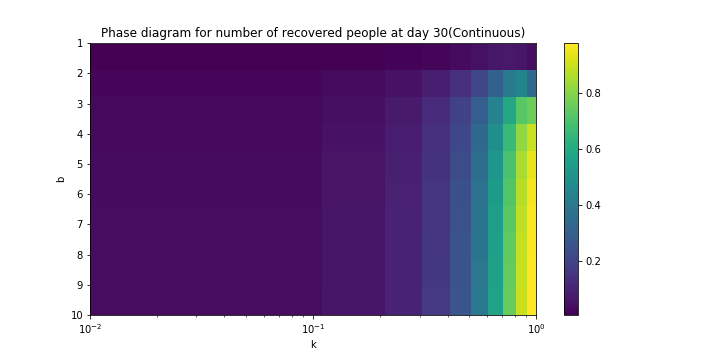
\includegraphics[width=.5\textwidth]{Phase_Continuous_R.png} & 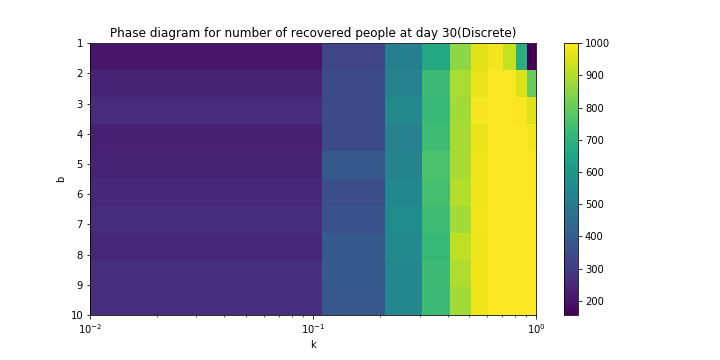
\includegraphics[width=.5\textwidth]{Phase_Discrete_R.png}
 	\end{tabular}
 
 \end{center}

\medskip \noindent
In terms of the recovery people at day 30, the diagram should be nearly the complement of the infected people diagram since people are only on this three stages in our model. From the first phase diagram, almost the no people are susceptible except the some cases mentioned. 


\subsection*{Spatial SIR model}
The idea for introducing spatial models is that in some cases, disease spreading is more localized, which means people usually interact with a specific group of people (in the work or family communities). Proposing spatial models can resolve this problem to some extent. 
\medskip \noindent \newline
Agent-based model:

\medskip \noindent
Based on the basic agent-based model we had above, we did some slight modification to get the spatial models. We first create a 2D position vector, then a person with random position can take a step of length $p$ in a random direction. After that, the people they interact with is all people surrounding by him with radius $q$. We used $KD$Tree from $Scipy$ package to achieve our goal. This way, we replaced parameters $b$ from our previous model since the use of $q$ describes numbers of interactions. 

\medskip \noindent \newline
PDE model: 
Alternatively, we can tackle spatial component in SIR model through partial differential equation(PDE). Solving PDE first we create the 2-dimensional finite difference Laplacian matrix L, and we discretize the square into an M * M grid. Then we turn this into a system of ODEs by vectorising the 2-dimensional arrays s, i and r. And we can get the following equations:

$\partial s(x, t)/ \partial t = -b \times s(x, t) \times i(x, t) + p \times L \times s(x, t)$

$\partial r(x, t)/ \partial t = k \times i(x, t) + p \times L \times r(x, t)$

$\partial i(x, t)/ \partial t = b \times s(x, t) \times i(x, t) - k \times i(x, t) + p \times L \times i(x, t)$

  \begin{center}
 	Figure 6: Relation between p and infected people(rate)
 \end{center}
 \begin{center}
 	
 	\begin{tabular}{c c}
 		\textbf{\underline{Discrete}} &
 		\textbf{\underline{Continuous}} \\
 		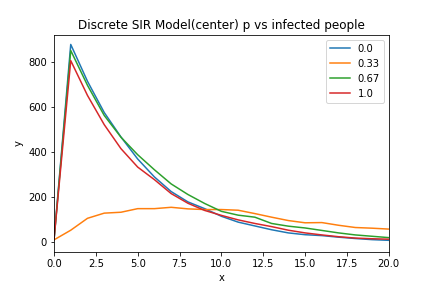
\includegraphics[width=.5\textwidth]{Discrte_spatial(center)_p.png} & 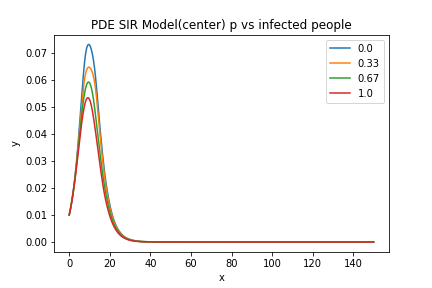
\includegraphics[width=.5\textwidth]{PDE(center)_p.png}
 	\end{tabular}
 
 \end{center}
 
\medskip \noindent \newline
The above figure shows the evolution of infected people(rate) changes as time increases, when $b=1, k=\frac{2}{3}$ and people initial position is at center. Both Continuous and Discrete model shows as p increases, the maximum infected people in a day decreases. This makes sense because as p increases, people are more likely to spread out, which lead to lower infected probability. 

  \begin{center}
 	Figure 7: Discrete spatial SIR with different initial position 
 \end{center}
 \begin{center}
 	
 	\begin{tabular}{c c c}
 		\textbf{\underline{Discrete(corner)}} &
 		\textbf{\underline{Discrete(center)}} &
 		\textbf{\underline{Discrete(random)}} \\
 		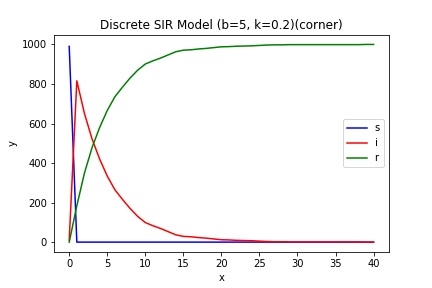
\includegraphics[width=.33\textwidth]{D_SIR_S_corner.png} & 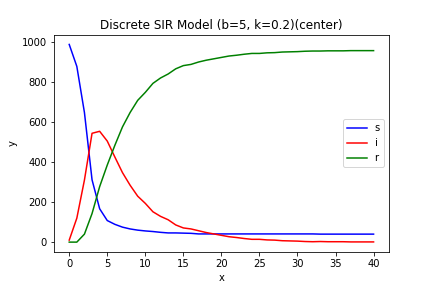
\includegraphics[width=.33\textwidth]{D_SIR_S_center.png}& 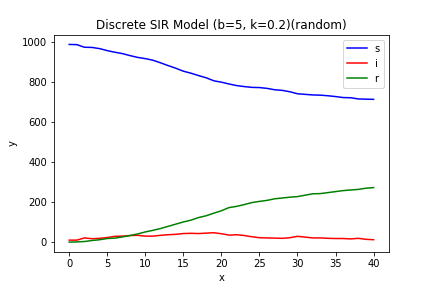
\includegraphics[width=.33\textwidth]{D_SIR_S_random.png}
 	\end{tabular}
 
 \end{center}

%\newpage
  \begin{center}
 	Figure 8: Continuous spatial SIR with different initial position 
 \end{center}
 \begin{center}
 	
 	\begin{tabular}{c c c}
 		\textbf{\underline{Continuous(corner)}} &
 		\textbf{\underline{Continuous(center)}} &
 		\textbf{\underline{Continuous(random)}} \\
 		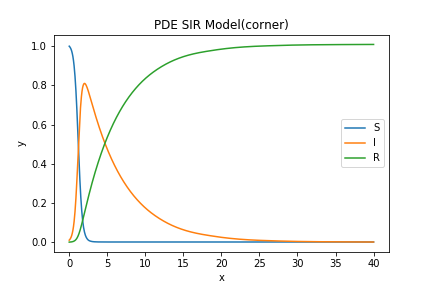
\includegraphics[width=.33\textwidth]{PDE(corner)_s.png} & 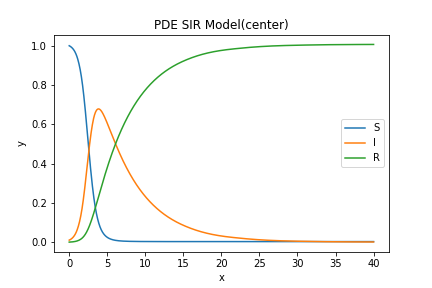
\includegraphics[width=.33\textwidth]{PDE(center)_s.png}& 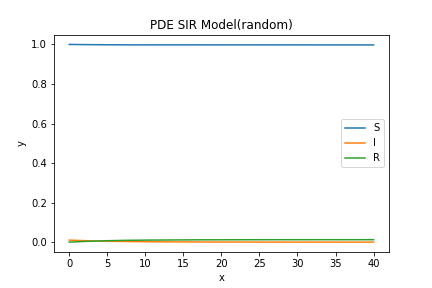
\includegraphics[width=.33\textwidth]{PDE(random)_s.png}
 	\end{tabular}
 
 \end{center}

\medskip \noindent
Both continuous and discrete model shows the peak of infected people(rate) is highest when the initial position is corner, then it follows by center and lastly random. This is because when people cluster at corner, they are more likely to be infected since the area is more dense and movements are restricted. people cluster at center has less restriction on movement, which lead to lower peak for the infected people(rate). The random starting position is not compact. Therefore, it has the lowest peak of infected people(rate). 

\subsection*{Variations investigations}
\subsubsection*{Model 1}
Assuming we want to investigate if reopening the elementary schools across the country is a wise choice or not, our basic SIR model can help us to determine the problem. According to the research, the average number of students per school for all elementary schools is 473 (Public Elementary Schools). This is used as our reference for the studies. The recovery rates is about 13.425 days for young people from 0 to 19 years old, which is calculated roughly by average of 13.61 day(male) and 13.24 days(female) (Voinsky et al.). By following a Poisson distribution with $\lambda$ = 0.074, we calculate the average daily recover rates $k$. In terms of number of contact people, this is the variable we are varying. 

\medskip \noindent
Consider the real situation that little children have limited self-disciplinary so we are not assuming they can obey the CDC guidelines such as wearing masks properly, or keeping the 6-feet away from others. Therefore, we used our basic SIR model to do this simulation. Since both continuous and discrete models are the basically the same, we randomly choose to implement the continuous model:


  \begin{center}
 	Figure 9: SIR Model vs Maximum Infected People as b Varies
 \end{center}
 \begin{center}
 	
 	\begin{tabular}{c c}
 		\textbf{\underline{SIR for b = 1, k = 0.074}} &
 		\textbf{\underline{Max infected people vs b}} \\
 		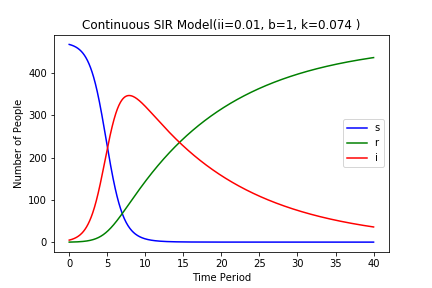
\includegraphics[width=7cm, height=5.2cm]{cont_b1.png} & 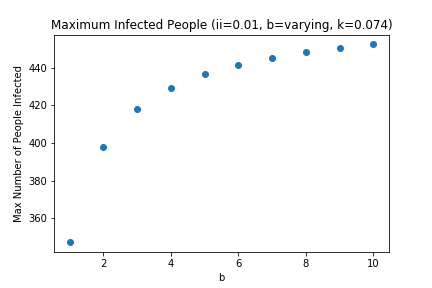
\includegraphics[width=7cm, height=5.2cm]{cont_peak.png}
 	\end{tabular}
 
 \end{center}
  


\medskip \noindent
From the left figure, when ii = 0.01, b = 1, k = 0.074, one clear observation is that we have a very tall, skinny curve for infected people with peak at around Day 7 for about 350 students, which is very bad. Why? Because this means many people get sick simultaneously and we do not have enough time to prevent to spread the disease (Gavin, 2020). 

\medskip \noindent
From the figure on the right, we can see that maximum number of infected people has an increasing trend as b increases, but as b gets larger, the curve becomes more stable. This result is not surprising since when we b = 1, the maximum infected people is already 350, which is 74\% of the total students, therefore, as b raises, the maximum infected people is limited, which shows an increasing trend. This plot is useful in a way to give information to schools about how many people will get infected at maximum if they do not do any actions when reopening the schools. 

%At the same time, it will also increase the burden for the hospital (ref). 



\subsubsection*{Model 2}
Reinfection is a situation when people are re-infected by a disease. This can occur when people are not immune to the disease. For some viruses, infection can provide lifelong immunity. For the other viruses, infection only provides temporary immunity, which could lead to potential reinfection. \emph{Tillett et. al} states the first confirmed case of severe acute respiratory syndrome coronavirus 2 (SARS-CoV-2) reinfection in the USA. This shows that reinfection could occur for some diseases. COVID-19 reinfection is still under investigation. \emph{Akiko} shows a evidence of COVID-19 reinfection, while \emph{Osmam et. al} shows previous negative results might be attributed to false-negative laboratory results and prolonged viral shedding, rather than to re-infection. Reinfection for COVID-19 is still debatable.

\medskip \noindent
In this model, we would investigate the possibility of COVID 19 reinfection. We would fit COVID-19 data to SIR ODE model, which includes reinfection component. 

\medskip \noindent
After we fit the data to the model, we could estimate the reinfected rate $r$. We would conclude there is evidence of COVID 19 reinfection if $r$ is greater than 0.05. 

\medskip \noindent
The implementation is completed in two steps: loss function and optimization. The loss function is defined as:
$$l(r)=||Susceptible_{data}-Susceptible_{simulation}||_2+||IandR_{data}-IandR_{simulation}||_2$$
\medskip \noindent
$Susceptible_{data}$ and $IandR_{data}$ is collected from United States Centers for Disease Control and Prevention. The data only contain total number of cases in United States, which is equivalent to total number of infected and removed in the SIR model. Therefore, we need to combine I and R for the loss function. Optimization is implemented through \emph{Scipy}. We fix number of days to be 319, initial infected percentage to be 0.01, then we can estimate $b,k,r$ through optimization. 

\medskip \noindent
Notice that for unconstrained optimization, the estimated values are $b=-0.00000966, k= -0.985, r=0.977$, which is impractical as $b$ and $k$ should be non-negative. One solution for this is to fix $k=0.074$ from model 1 and $b=0.0001$ for simplification. 


  \begin{center}
 	Figure 10: Figures for reinfection model
 \end{center}
 \begin{center}
 	
 	\begin{tabular}{c c}
 		\textbf{\underline{Loss Function}} &
 		\textbf{\underline{Covid SIR model vs data}} \\
 		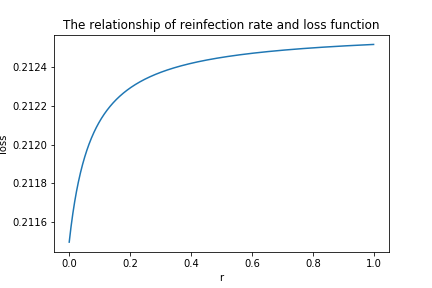
\includegraphics[width=7cm, height=5.2cm]{rvsloss.png} & 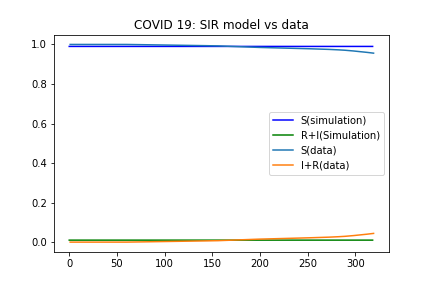
\includegraphics[width=7cm, height=5.2cm]{modelvsdata.png}
 	\end{tabular}
 
 \end{center}
 
%\begin{comments}
%\begin{center}
 %	Figure 10: Loss Function
% \end{center}
 %\begin{center}
%	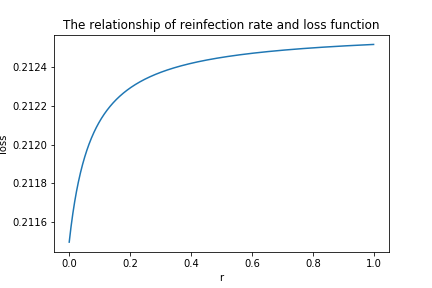
\includegraphics[scale=0.5]{rvsloss.png}
%\end{center}
%(put figure rvsloss here)
%\end{comments}

\medskip \noindent
When we fix $b=0.0001$ and $k=0.074$, we can get the above plot by obtaining the loss through manipulate $r$. The figures show as reinfection rate decreases, the loss function also decreases. This implies there is no evidence of COVID 19 reinfection.
\medskip \noindent


 %\begin{center}
 %	Figure 11: Covid SIR model vs data
 %\end{center}
%\begin{center} 
%	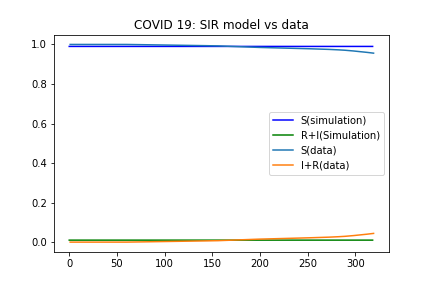
\includegraphics[scale=0.5]{modelvsdata.png}
% \end{center}
%(put figure modelvsdata here)



\medskip \noindent
This figure shows SIR simulation with$b=0.0001$, $k=0.074$ and $r=0.01$ vs COVID 19 data in the United States. The simulated SIR model fits well with the data before 200 days. The model fails to capture increase trend of infected and removed people in the United States after 200 days. Therefore, there are some room of improvement for SIR model.

\subsubsection*{Model 3}
It is obvious that people wearing masks can slow down the disease spread (Cooper et al). Therefore, we could implement the effect of the use of masks into the SIR model. For ODE model, we can implement it by reducing the parameter b. We can obtain data to calculate the effect of the use of masks on the number of interactions each day that could spread the disease (C, MacIntyre, et al). Thus, we can judge whether the use of masks can slow down the spread of the virus.

\medskip \noindent
We know that in Cooper’s paper, the authors conducted a prospective cluster-randomized trial(Cooper et al). During the 2006 and 2007 winter seasons, 286 exposed adults from 143 households were recruited. They found that during a severe pandemic when use of face masks is greater, pandemic transmission in households could be reduced.

\medskip \noindent
We introduce a new parameter q (0<q<1) to reduce the parameter b, then we can get the following equations:

$$\frac{ds}{dt} = -b \times s(t) \times i(t)$$
$$\frac{dr}{dt} = k \times i(t)$$
$$\frac{di}{dt} =  b \times q \times s(t) \times i(t) - k \times i(t)$$
\noindent
We have the parameter b = 1/2, k = 1/3 and the initial condition s = 0.99, r = 0, i = 0.01. From the figure shown in Appendix, we know that when we use surgical mask, q $\approx$ 0.83. And when we use P2 mask, q $\approx$ 0.74.





  \begin{center}
 	Figure 11: Different mask conditions
 \end{center}
 \begin{center}
 	
 	\begin{tabular}{c c c}
 		\textbf{\underline{Surgical masks}} &
 		\textbf{\underline{P2 masks}}  \\
 		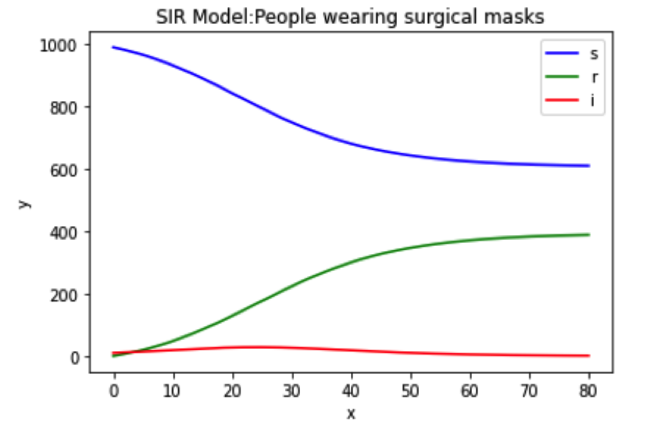
\includegraphics[width=.5\textwidth]{surgmask.png} & 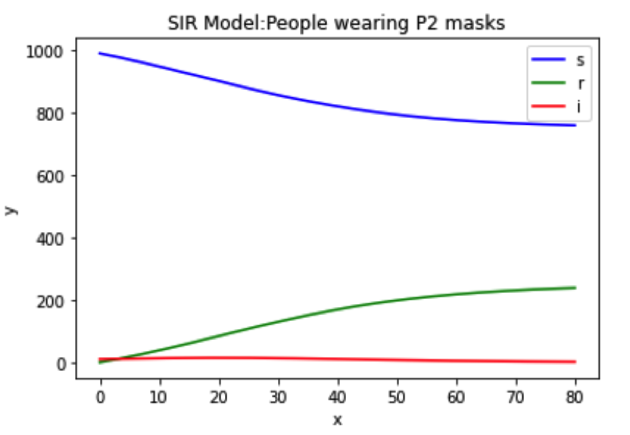
\includegraphics[width=.5\textwidth]{p2mask.png}
 	\end{tabular}
 
 \end{center}


\begin{center}
    \begin{tabular}{c}
    	\textbf{\underline{No masks}}  \\
	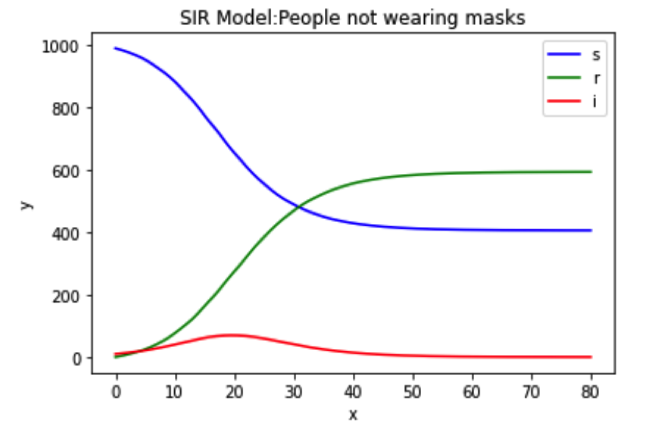
\includegraphics[scale=0.8]{nomask.png}
\end{tabular}
\end{center}
From the plot above, we know that the use of masks can slow down the spread of the virus from seeing there is a small peak at Day 20 while we do not observe that in the cases of wearing mask. In addition, we can compare with the P2 masks and surgical masks and we can get the conclusion that people wearing P2 masks is better than wearing surgical masks since the infectious curve is more flat in P2 mask situation.

\section*{Conclusion}	
%\subsection*{Summary to the results}
To conclude, our basic SIR models in 1D and 2D provide us with clear understanding about how many people will be infected/recovered during a specific period of time by manipulating variables. Both models indicate that as b increases, the peak for infected people takes place much earlier. When recovery rate raises, infected people drops since more sick people recovered from disease so they are not infectious anymore as well. 

\medskip \noindent
Spatial models add more dynamic to the SIR model. We observe from different starting position, the resulting model will be noticeably different. Parameter p also affects the model significantly. As p increases, the maximum infected people(rate) decreases. One limitation of the spatial models is there are some randomness involve in the discrete model, which leads to some fluctuation in the figures. One could address this by implement Monte Carlo method, which can tackle randomness effectively. 

\medskip \noindent
According to what we investigated above for model 1, it is dangerous to reopen the school at this point, if students cannot strictly follow the public health guidelines. Even with just the initial infectious people is 0.01, and each student interact with 1 other, 74\% of the students in the school will get sick at Day 7, which is a very scary result. One improvement can be considered with this model is that we haven't consider the factor that sick students are not allowed to go back to school. This will slow down our results of infected people since they will not interact with other students.


\medskip \noindent
For SIR model with reinfection component, we show that there is no evidence of COVID 19 reinfection. For continuous model, the reinfection rate is fixed. This neglects that fact that immune system enhance after people are recovered from diseases. Vaccine is am example for this. Discrete model addresses this issue by decreasing reinfection rate when people recover. However, there is no simple solution for continuous model. 

\medskip \noindent
In terms of the third model, we can generate the following two conclusions. First, the use of masks can slow down the spread of the virus. Moreover, people wearing P2 masks is better than wearing surgical masks. A limitation here is that this trial only compared the effects of two masks and we can also compare the effects of various masks to determine which mask works best. In addition, we can introduce a new parameter d to increase the social distance between people to slow down the spread of the virus, which can make the model more complete.




%\subsection*{Limitations}



\newpage

\section*{Bibliography}

1. C, MacIntyre, et al. “Face mask use and control of respiratory virus transmission in households.” National Library of Medicine. Published by National Center for Biotechnology Information., 
Feb. 2009, https://pubmed.ncbi.nlm.nih.gov/19193267/. 

\medskip \noindent
2. Cooper, Ian, et al. “A SIR model assumption for the spread of COVID-19 in different communities.” Chaos Solitons Fractals. Published by Elsevier Ltd., Oct. 2020, https://www.ncbi.nlm.nih.gov/pmc/articles/
PMC7321055/. 


\medskip \noindent
3. Gavin, K., 2020. Flattening The Curve For COVID-19: What Does It Mean And How Can You Help?. [online] Healthblog.uofmhealth.org. Available at: <https://healthblog.uofmhealth.org/wellness-prevention/flattening-curve-for-covid-19-what-does-it-mean-and-how-can-you-help> [Accessed 8 December 2020].

\medskip \noindent
4. Osman A.A. and Al Daajani M.M. and Alsahafi A.J. (2020). Re-positive coronavirus disease 2019 PCR test: could it be a reinfection? {\it New Microbes and New Infections} (37)

\medskip \noindent
5. Public Elementary Schools, by Grade Span, Average School Size, and State or Jurisdiction: 2005-06. National Center for Education Statistics, U.S. Department of Education,

\medskip \noindent
6. Tillett R.L., Sevinsky J.R., Hartley P.D., et al. (2020). Genomic evidence for reinfection with SARS-CoV-2: a case study. {\it Lancet Infect Diseases}; 

\medskip \noindent
7. Iwasaki A. (2020). What reinfections mean for COVID-19. {\it The Lancet Infectious Diseases}. 

\medskip \noindent
8. Voinsky, Irena, et al. “Effects of Age and Sex on Recovery from COVID-19: Analysis of 5769 Israeli Patients.” The Journal of Infection, The British Infection Association. Published by Elsevier Ltd., Aug. 2020, www.ncbi.nlm.nih.gov/pmc/articles/PMC7229949/. 





\newpage
\section*{Appendix}

  \begin{center}
 	Figure 1: Summary statistics of wearing/no wearing masks
 \end{center}
\begin{center} 
	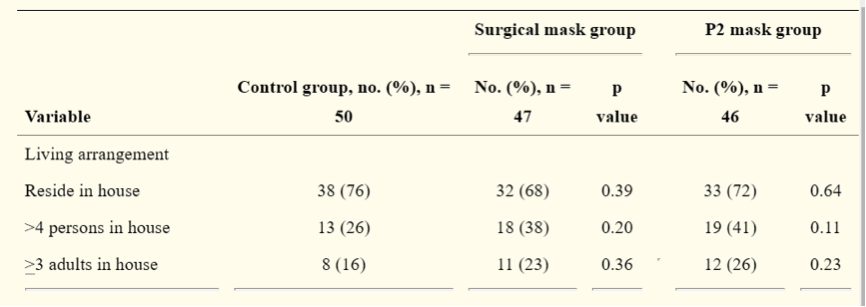
\includegraphics[scale=0.9]{maskov.png}
\end{center}
Citied: C, MacIntyre, et al. “Face mask use and control of respiratory virus transmission in households.” National Library of Medicine. Published by National Center for Biotechnology Information., 
Feb. 2009, https://pubmed.ncbi.nlm.nih.gov/19193267/. 

\end{document}